\chapter{Implementation}
\label{IMPL}
Our implementation uses the MVC structure to create a practical class design. We
have prioritized to make our design as simple and intuitive as possible. We used
object oriented principles to assure that our design has both low connection
between classes (loose coupling), and a high degree of cohesion.

By following these principles we have achieved implementation with minimal code
duplication and with good possibility for extension.

Some of the basic thoughts on our design is explained in figure
\ref{fig:BasicDesign}, and \ref{fig:PathfindingStructure}.

\begin{figure}[h!]
\centering
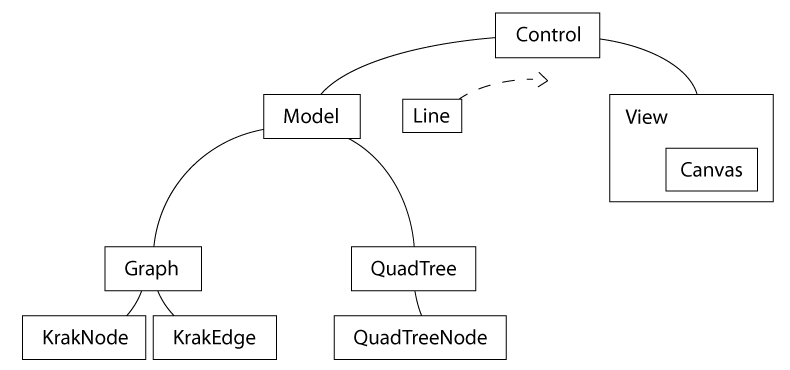
\includegraphics[width=1\linewidth]{images/BasicDesign}
\caption{The basic design of our implementation. The controller gets a
collection of lines, that the view will draw.}
\label{fig:BasicDesign}
\end{figure}

\begin{figure}[h!]
\centering
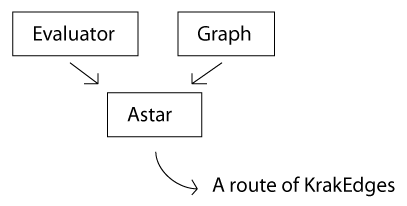
\includegraphics[width=0.5\linewidth]{images/PathfindingStructure}
\caption{The pathfinding part of our implementation. The static A* function
takes an Evaluator and a Graph and returns a path.}
\label{fig:PathfindingStructure}
\end{figure}

This rest of this chapter describes how we have implemented some of the more
interesting features of the software. We aim to describe it to enough detail that this
chapter can serve as a guideline for implementing the functionalities we
describe.

\section{UTM-conversion}
\label{IMPL-UTM}
When the graphical user interface part of the map tries to communicate with the
model through control, some conversions of the different kind of values are
necessary. Both when going from coordinates in the java-coordinate system to
UTM32-coordinates and back.

We need to convert the values when we want to use the mousezoom and when we want
to place the markers for pathfinding. We get an input on the graphical user
interface when we mousezoom and this needs to be converted to UTM-coordinates so
that we can create the new boundaries of the zoomed rectangle.

When we place markers for pathfinding, we do the same as when we do mousezoom,
but instead we store the point as UTM32-coordinates and whenever we move the
map, we convert it back to pixel-coordinates so that we know where to draw.

The java-coordinates have origo in the top left corner with the y-coordinate
increasing the further down the y-axis you go. UTM32-coordinates are a bit
different. UTM32 has origo in the bottom left corner and the y-coordinate
increasing the further up you go on the y-axis.

% Re-phrasing needed probably.
We have a utility class with methods for converting the points back and forth.
One takes a point from the view. The model and the view itself a formula
for converting the pixelpoint to the UTM32-point.

Below is an illustration of the conversion from pixel to UTM.

\begin{figure}[!ht]
\centering
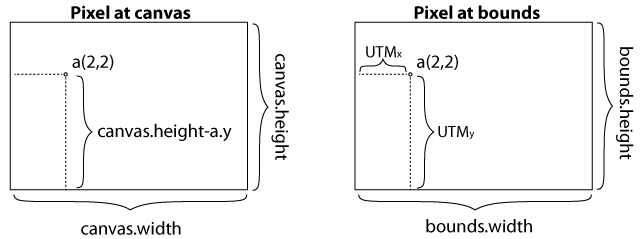
\includegraphics[width=1\linewidth]{images/UTMillu}
\caption{Illustration of UTM conversion}
\label{fig:UTMconversion}
\end{figure}

We click on a point, 'a', on the canvas. To calculate the the UTM coordinate
corresponding to that point, we use the formulas:

$
UTM_x = bounds_x + \cfrac{a_x}{canvas_{width}} \times bounds_{width}\\
\\
UTM_y = bounds_y + \cfrac{canvas_{height} - a_y}{canvas_{height}} \times bounds_{height}\\
\\
$

To convert from UTM to pixels, we use the same formulas but reversed:

$
\\
Pixel_x = \cfrac{(a_x - bounds_x)}{bounds_{width}} \times
canvas_{width}\\
\\
Pixel_y = canvas_{height} - \cfrac{a_y - bounds_y}{bounds_{height}} \times
canvas_{height}\\
\\
$

\section{Mousezoom}
\label{IMPL-MZ}
We have implemented the mouse zoom requirement by using \class{mouseEvent}s on
our canvas. When the user presses the left mouse button down, it generates a
\class{mousePressed} event. We record the position of the mouse at the time of
the \class{mousePressed} event and wait for the \class{mouseReleased} event.
When the left mouse button is released, it generates a \class{mouseReleased}
event. We use the positions of the mouse at the \class{mouseReleased} event and
the \class{mousePressed} event to calculate new bounds for the model.

% Redundant?
As mentioned in section \ref{IMPL-UTM} \class{\nameref{IMPL-UTM}}, we use
UTM-conversion to convert pixel values into the UTM values we need.

% This paragraph can probably be longer and more detailed.
Often the user will not drag a square that is in perfect ratio with the
canvas. If it does not have the same ratio as the canvas, we change the ratio
of the dragged square behind the scenes. We do this by either adding length or
width to the dragged square. We always make sure to at least show what was
inside the box the user dragged.

If the ratio of the dragged square is smaller than the canvas ratio, we make the
dragged box wider. If the ratio of the dragged square is larger, we make the
dragged box taller.

\section{Dijkstra vs A*}
\label{IMPL-DVA}
When planning the pathfinding feature, we had to decide between two algorithms:
Dijkstra and A*. The latter is based on Dijkstra, but achieves better performance by
using heuristics.

% First sentence should be re-phrased.
The Dijkstra algorithm uses a minimum priority queue to find the shortest path
from a given node to every other node by looking at the edges connecting nodes.
The program will take a node from the priority queue and add all the other nodes
that are connected to the current node to the priority queue. The priority queue
stores a value with the node, which is the distance to the current node
plus the length of the edge between the two. Since the priority is made to return
the node with the smallest value associated with it, the next node in line will
always be the one which is closest to the start node. This procedure continues
until all nodes have been visited and by logging what edge led to all the nodes,
it is possible to trace back the route to the start node.

This algorithm is great if we need to find the distance from one point to many other
points, but can be quite slow when using it for finding a path between to nodes,
since it just searches in all directions without thinking about in which direction the
target node is.

% ``estimated distance ... the given node'' - should be more clear.
This is where A* comes in handy. The A* algorithm is a modification of Dijkstra's
algorithm that also looks at the estimated distance from the given node when
determining the value for the priority queue. When using the geographical distance
as a measure of best route, the value would be the current distance from the start
node plus the direct distance to the target (as if there were a road directly to
the target). With this subtle change, the algorithm will prioritize nodes that are
relatively closer to the target rather than those that are in the other
direction. This makes the algorithm much faster since it will not pay much attention
to the roads that are not in the direction of the target.
We have decided to use the A* algorithm since we only calculate routes between
two distinct nodes and therefore don`t need the route from the start node to all
others. The time reduction that A* gives is also a definite plus since no user
wants to sit and wait too long for the program to find a route.

\begin{figure}[!ht]
\centering
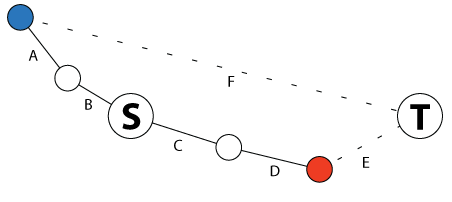
\includegraphics[width=1\linewidth]{images/AstarVSDijkstra.png}
\label{}
\caption{A* vs. Dijkstra example. The dashed lines are the direct distances,
used by A*. The Dijkstra algoritm will check the blue node before the red
node, because B+A \textless C+D. The A* algoritm will check the red node
before the blue node, because C+D+E \textless B+A+F.}
\end{figure}

The smaller the difference from the direct distance is to the actual fastest
possible route, the more we will benefit from the A* algoritm. This
difference will often be bigger for the routes calculated for the car. This is
because the fastest route would be a straight highway, which often is far from
possible. We can therefore conclude that the A* algoritm typically is more
of a benefit when calculating routes for bicycling because they rely on the
distance.

\section{Evaluator}
\label{IMPL-EVA}
In order to make our path finding algorithm flexible enough for different 
interpretations of the ``best route'', we have added an entity called \class{Evaluator}. 
This is an object that has the responsibility of evaluating a node relative to 
the target node. 

The \class{Evaluator} also has the responsibility of calculating the 
heuristics that the A* algorithm relies on. By using the \class{Evaluator} we are able to 
use the same path finding algorithm for two very different tasks; the biking route and 
the car route. The major difference between these is that the bike's heuristics is based 
on the distance, where as the car's heuristics is based on the total drive time. 

\begin{center}
$
dist(p_{1},p_{2})=\sqrt{(x_{1}-x_{2})^{2}+(y_{1}-y_{2})^{2}}
$
\end{center}

\begin{center}
$
time_{drive}=\frac{dist(p_{1},p_{2})}{1000\cdot \frac {speed_{max}}{60}}
$
\end{center}

We use these formulas to calculate the heurestics for bike routes, car routes respectively.
There are currently three three different evaluators in the program as static variables. These
are called BIKE, CAR and HAS\_NAME. The HAS\_NAME evaluator is used when getting
the name of the road closest to the mouse. There is also a fourth variable called DEFAULT that is a help to
any future developers if they are unsure of what to use, this variable is currently just refering
to CAR. 

The Evaluator implementation is a good example of making our code ready for future features, 
since if we needed to add other means of transportation or simply variations of the ones 
we have, we would only need to create new \class{Evaluator}s and not change 
a single line of code in the A* algorithm.

\section{Quadtree}
\label{IMPL-QT}
% Quadtree, serialization and threading should maybe be in its own section
% (called optimizations or something)
% This section reminds me of a lot of different statements, not really joined together.
% Needs more pros and cons, and should be ``longer'' / more in depth.
In order to improve the drawing of our map, we have implemented a data structure
called quadtree. The quadtree divides our map in four squares. In these four squares
it divides our roads again into smaller squares, and we keep doing this, until we reach
an amount of roads that is manageable.
When we want to retrieve data from the map, we can give the quadtree a
rectangle, and it will return all the roads within our smaller squares that intersect
that rectangle. This technique optimizes the drawing of the roads, because we
limit the amount of roads we draw.

However, when viewing the entire map of Denmark, this implementation does not help
us. Therefore, it is necessary to only to draw the bigger roads when zoomed out. We
have discussed two different techniques to do this.

The simplest solution would be to iterate over the roads returned and then
remove the road we do not want to draw. However, it would be more efficient to sort the
roads before we put them in the quadtree, and then have them sorted in the quadtree.
With this method we will not to iterate and remove the roads all the time.

\begin{figure}[h!]
\centering
\includegraphics[width=1\linewidth]{images/UnsortedQuadtree.png}
\caption{Unsorted Quadtree. A quadtree were the roads are not sorted. The
dashed lines are parts of the quadtree that we do not show for practical
reasons.}
\label{IMPL-USQ}
\end{figure}

We have discussed two different ways to sort the roads in the quadtree.

The first technique relied on dividing the types of roads into different quadtrees.
With this implementation, we only implement the quadtrees containing the roadtypes
we want to draw, into our drawing. See figure \ref{IMPL-DCMQ}.

\begin{figure}[h!]
\centering
\includegraphics[width=1\linewidth]{images/MultiQuadtree.png}
\caption{Multiple quadtrees. The user can choose which quadtrees to run
through.}
\label{IMPL-DCMQ}
\end{figure}

The second technique relied on putting the bigger roads at the top of the
quadtree when building it. Then we could specify at which depth we wanted to
search the quadtree. We called this 'the depthcontrolled quadtree', see figure
\ref{IMPL-DCDQ}.

\begin{figure}[h!]
\centering
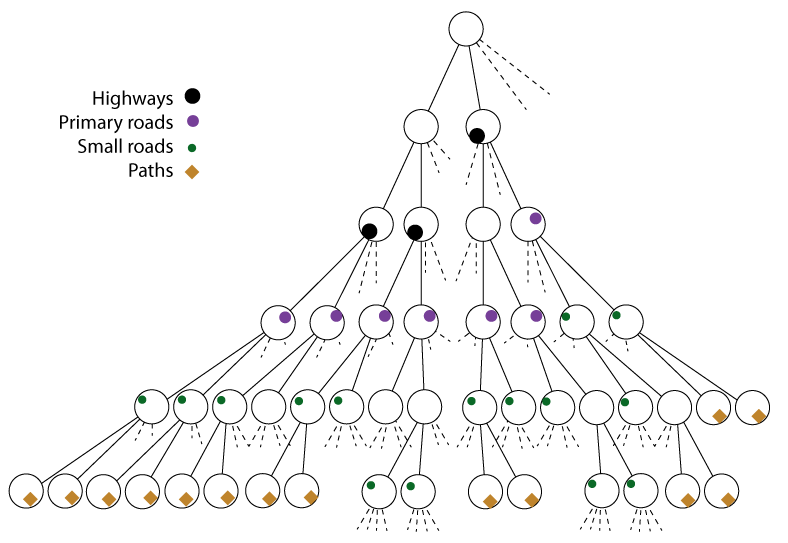
\includegraphics[width=1\linewidth]{images/DepthcontrolledQuadtree.png}
\caption{The depthcontrolled quadtree.}
\label{IMPL-DCDQ}
\end{figure}

The two methods both have advantages and disadvantages.

The depth controlled quadtree would return more roads than the multiquadtree,
because the big roads would lie in big rectangles, and therefore be drawn more
often.

The depth controlled quadtree requires less RAM than the multiquadtree,
because it requires less instances of object QuadTreeNode.

The multiquadtree is less efficient to search through than the
depthcontrolled quadtree, because we must run through each quadtree
individually.

Looking at the advantages and disadvantages of these quadtrees, we have chosen
to implement the multiquadtree. We have done this because it is the drawing of
the roads that slows our implementation. The efficiency of our program is not
affected by the efficiency of the quadtree search. The efficiency of the map is
affected because of the number of roads drawn.

\section{Serialization}
\label{IMPL-SERI}
We observed that the user had to wait quite a long time for the program to start. This
was because every time we start the program, we loop through the entire dataset given
to us by Krak. This data-set is huge, and because of this it takes quite a lot of time to
start the program. Because we need to load all these data, the user is presented with
a blank screen for a long time, before all these data are loaded and the program starts.

We started looking for a way to speed up the loading process, so the user has a map in
front of him or her quickly, when the user starts the program. What takes the most time
is looping through the data and creating the needed datastructures (quadtrees, the
graph and so on), so if we could skip these steps or speed them up, we could save a lot
of time.

This is where serialization comes into play. By serializing an object, you transform your
object into something that can be passed around, through streams and such. So by
serializing objects, you can save them to files. If the object to be serialized contains
references to other objects, these will also be serialized (if they are Serializable /
implements java.io.Serializable).

By doing this, we only need to build our datastructures the first time you start the program.
After the objects have been created, they are been serialized and saved to files. The next
time the user starts the program, we check whether the data has been changed. We check
this by checking the MD5 checksum of the file, with
\class{MD5Checksum}\footnote{We borrowed this code from \cite{MD5}} (we didn't
write this class ourselves). When we serialize the objects, we also save the checksum to a config file. If the data hasn't been changed (i.e. the checksum is the same), we load the objects that
we saved, instead of making them all over.

We serialize all the quadtrees, the graph and the maxbounds-object (specifying the bounds
of Denmark), as these are the objects we need for the program to run. When saved to the
harddrive, it is around 65MiB, which is okay, given the sizes of harddrives today.

We save all these objects to one single file, in order to keep the references. If we didn't do
this, the references will be ruined, which can break the program. We experienced problems
with this, as nodes and edges is both stored in the quadtrees and the graph. If we serialized
and saved the quadtrees in one file, and the graph in other file, a given node will be saved
twice, and when we load the data from the serialized files, the node will exist twice, and it
won't be the same node. But if we save the objects to a file through the same stream, we only
get one of each, which leads to less RAM usage, less harddrive usage, faster loadtimes and
fewer bugs.

\subsubsection{Threading}
By serializing our main objects, we cut several seconds of our load times. But we can do it
even faster. We are serializing several objects, but only few of them are needed right from
the start of the program. So what we can do to speed it up even more, is loading the few
necessary objects, and then load the rest in the background. We do this with threads.
We load the few objects we need from the start, then create a new thread to load the rest
of the objects, and in the mean time, we create the window and draw the map.

The same goes for the first run. The user doesn't need to wait for the program to finish
serializing and saving to files. By using threads, we can create the datastructures, and
then immediately show the window to the user, while saving the objects to files in the
background.

During load time (when loading from the serialized files, after the window is shown to the
user) not all quadtrees are loaded. So we did encounter a problem when querying the
quadtrees, when not all of them were loaded. We solved this by putting the querying in
a try/catch, and when a problem occurred (index out of bounds, when trying to access a
quadtree not yet loaded), we simply stopped looking through more quadtrees and just
return what we found so far. Then later on, when all quadtrees were loaded, we could
return all edges. The user wouldn't notice the lack of roads, as the user only sees a limited
amount of roads anyway.

We did encounter another problem, when trying to use the graph (for pathfinding) when the
graph wasn't done loading. We solved this by using a simple loop, that check if the graph was
set. As long is the graph wasn't available, the main thread would simply hold and wait for the
loading to finish. This is probably the only time where the user would notice that everything isn't
quite loaded, but the loading happens so fast, that it probably won't be a problem anyway.
